\begin{apendicesenv}
	\chapter{Como fazer uma rede neural}
	
	\section{Entendo aproximadores de função}
		\begin{itemize}
			\item Analisar o contexto do problema: O mesmo é linear, não linear \cite{rashid2016make}.
			\item A partir do item anterior, definir qual a função da ativação será usada \cite{rashid2016make}.
		\end{itemize}
	
		\par É importante também, dependendo do tipo de problema, saber escolher uma função de cálculo de erro, essa função, pode ser uma função quadrática, linear ou outra dependendo da importância que o erro tem na solução do problema. As funções de cálculo de erro mais usadas são mostradas abaixo:
		
		%TODO Colocar  exemplos de função de cálculo de erros
		\begin{itemize}
			\item $erro = valorDesejado - valorCalculado$
			\item 
		\end{itemize}
	
		\par Calculado o erro é necessário agora, de alguma forma, fazer com que esse erro seja corrigido utilizando uma abordagem iterativa que se aproxima cada vez mais do valor desejado usando pequenos passos. Considerando que $\Delta$ represente uma pequena variação em um valor $peso$, e sendo  $peso$ um dos parâmetros da função de ativação de um aproximador ($y = peso . x$ para uma função de ativação linear) então temos que a correção do valor deve ser dado como na equação abaixo:
		
		\begin{equation}
			valorDesejado = (peso + \Delta peso) . entrada \qquad,
		\end{equation}
		\cite{rashid2016make}
		
		\par Então, sabendo que o $valorDesejado = peso + \Delta peso . entrada$ e que $erro = valorDesejado - valorCalculado$ se pode concluir que:
		
		\begin{equation}
			\Delta peso = \dfrac{erro} { entrada} \qquad,
		\end{equation}
	
		\par No tocante as funções de ativação se pode imaginar quantas forem necessárias, no entanto, algumas se destacam dentro do campo das redes neurais:
	
		\begin{itemize}
			\item \textit{step function}: \begin{equation}
				y = \begin{cases} 
					0 & x\leq 0 \\
					1 & x > 0 \\
				\end{cases}
			\end{equation}
			\item \textit{sigmoid function}: \begin{equation}
				y = \dfrac{1}{1 + e^{-x}}
			\end{equation}
			%TODO Apresentar outro exemplos de função de ativação
		\end{itemize}
	
		\par No entanto, existe um problema quanto a esta abordagem, a função de ativação que recebe o parâmetro $peso$ Se adaptará ao último exemplo mostrado a ela criando uma situação conhecida como "overfitting", invalidando assim todos os os outros exemplos anteriormente usados, portanto, como se pode notar, é necessário a criação de um elemento que impeça esse ajustamento extremo, chamado de taxa de aprendizado:
		
		\begin{equation}
			\Delta peso = taxaDeAprendizado . \left( \dfrac{erro} { entrada} \right) \qquad,
		\end{equation}
			
		\par Usualmente a taxa de aprendizado é um valor suficientemente pequeno cujo o objetivo é garantir que o \textit{ovefitting} não aconteça mas, suficientemente grande para que a rede aprenda em um tempo razoável. Sendo $0,1$ um dos valores normalmente usados.
		%TODO Não citar redes neurais nessa sessão
		
		
		%TODO citar as referências para es "outres autores" citades no texto abaixo
		\par Já outros autores preferem usar uma função de erro "acumulada", desta forma, o erro é calculado em lote segundo várias entradas e saídas processadas pela rede de forma que se compute o erro acumulado segundo a expressão \ref{eq:batchError} onde $E$ é o erro $M$ é o tamanho do vetor de saída da rede, $N$ é a quantidade de amostras fornecidas, $y_{ik}$ é o vetor de resultante da rede e $t_{ik}$ é o vetor esperado.
		
		
		\begin{equation}
			E = \dfrac{1}{2MN} . \sum_{k}^{N}\sum_{i}^{M}(y_{ik}-t_{ik})^2 \qquad,
			\label{eq:batchError}
		\end{equation}
		
	\section{Junção dos aproximadores: Redes neurais }
		\par Já que a sessão anterior definiu o que é um aproximador de funções, nesta sessão, usando as definições já vistas, será apresentada a definição de uma rede neural que é a junção de vários aproximadores que, dessa forma, conseguem  delimitar espaços de resultados mais complexos além daqueles que podem ser separados por apenas uma função de ativação.
		
		\par Um dos exemplos clássicos que necessitam dessa abordagem mais complexa é o exemplo da porta lógica \textit{xor}. Quando se tenta usar apenas um aproximador de funções para conseguir os resultados dessa porta é possível notar que o mesmo não é capaz de criar um espaço de resultados suficientemente complexo afim de separar os pontos fornecidos, sendo assim, Torna-se necessário o uso de múltiplos aproximadores (ou, nesse caso, 2).
		
		\par Pode-se considerar tal junção como uma a rede neural. É possível perceber que a mesma passa ter múltiplas entradas tornando-se necessário, antes que a função de ativação seja aplicada, que a soma dessas entradas seja feita. A este procedimento se dá o nome de \textit{feedforward} \cite{haykinredes}:
		
		\par Via de regra uma rede neural tem, no mínimo, duas camadas: A camada de entrada que é usada apenas para representar os valores que serão processados e a camada de saída, cujo papel é fazer a soma ponderada das entradas passando então o resultado dessa operação para uma função de ativação que finalmente gerará as saídas de nossa rede neural como ilustrado na figura \ref{fig:simpleNeuralNetwork}.
		
		\begin{figure}[H]
			%TODO Fazer a figura de uma rede neural simples
			\centering
			\caption[Uma rede neural simples Fonte: O autor]{Uma rede neural simples Fonte: O autor}
			\label{fig:simpleNeuralNetwork}
			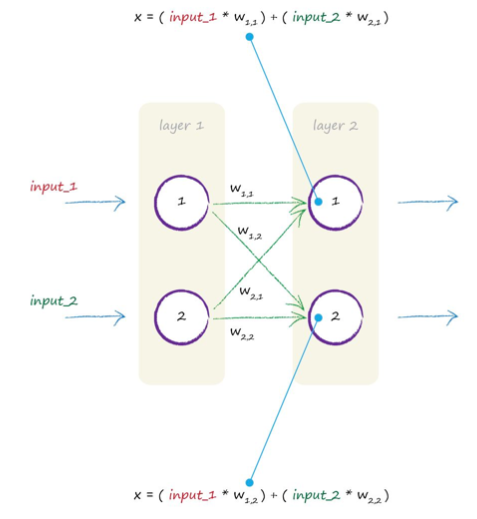
\includegraphics[width=0.7\linewidth]{images/TEMPSimpleNN}
		\end{figure}		

	\section{Uma rede neural simples}
		\par Como visto na figura \ref{fig:simpleNeuralNetwork} da sessão anterior uma rede neural conecta suas camadas usando pesos que servirão como moderadores das entradas da próxima camada com o fim desse evitar o \textit{overfitting}. É possível representar uma rede neural de várias formas, no entanto, como ilustrado na figura \ref{fig:matrixmultnn}, a forma mais eficiente computacionalmente será a matricial, usando esta abordagem será possível representar facilmente as camadas e os respectivos pesos que as ligam, melhorando também o desempenho computacional já que tais operações são altamente paralelizáveis.
		
		
		\begin{figure}[H]
			\centering
			\caption[Representação de uma rede neural usando matrizes]{Representação de uma rede neural usando matrizes}
			\label{fig:matrixmultnn}
			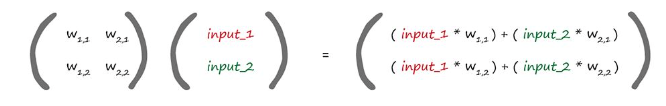
\includegraphics[width=0.7\linewidth]{images/TEMPMatrixMultNN}
		\end{figure}
		
	\section{Redes neurais multicamadas}
		\par A depender da complexidade do problema apenas duas camadas não são suficientes para que este aproximados universal de funções, mais conhecido como rede neural, consiga obter resultados satisfatórios. Assim, se torna necessário adição de uma ou mais camadas que servirão para aumentar a complexidade do espaço das soluções de nossa rede.
		
		\par Então, considerando o contexto, as tais camadas que devem ser adicionadas serão chamadas de ocultas ou \textit{hidden layers}\cite{rashid2016make}. 
		
		\par Em redes neurais multicamadas surge um novo problema: Como atualizar os valores dos pesos entre as camadas já que o erro produzido depende das várias entradas da camada anterior? Como mostrado na figura \ref{fig:simpleNeuralNetwork} o valor da próxima camada depende da soma ponderada pelos pesos dos valores da anterior sendo que tal soma deve passar por uma função de ativação escolhida, portanto, após o cálculo do erro na resposta da rede é preciso recalcular os pesos de forma a distribuir esses erros usando um algoritmo ao qual daremos o nome de retro-propagação ou \textit{backpropagation} \cite{haykinredes}. É importante frisar que este é apenas um dos vários métodos de treinamento da rede neural, é possível, por exemplo, usar uma abordagem bio-inspirada e/ou evolutiva.
		
		\begin{figure}[H]
			\centering
			\caption{Retro-propagação}
			\label{fig:backpropagation}
			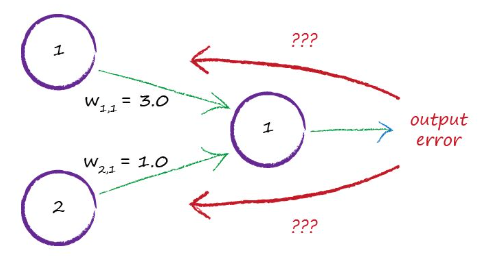
\includegraphics[width=0.7\linewidth]{images/TEMPbackpropagation}
		\end{figure}
	
	\section{Retro-propagação}
		\par Primeiramente é importante notar que os pesos associados a cada item da camada (neurônio) Contribuem com o erro resultante de forma proporcional aos seus respectivos valores, sendo assim, é necessário, ao fazer a retro-propagação, que esses erros sejam distribuídos proporcionalmente como indicado na figura \ref{fig:backpropagationErrors}.
		
		\begin{figure}[H]
			\centering
			\caption{Parcela da distribuição do erro na retro-propagação para o $erro_1$, o mesmo deve ser feito para todos os outros erros.}
			\label{fig:backpropagationErrors}
			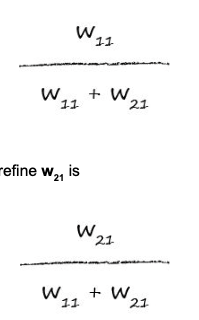
\includegraphics[width=0.4\linewidth]{images/TEMPbackpropagationErros}
		\end{figure}
		
		\par Calculada a parcela da participação de cada peso nos erros produzidos possibilta calcular o erro resultante na camada oculta, usando o mesmo raciocínio de cálculo da participação no erro, é possível continuar com algoritmo de retro-propagação. Assim, o cálculo do erro da camada oculta se dá como mostrado na equação \ref{eq:hiddenLayerError}.
		
		\begin{equation}
			\label{eq:hiddenLayerError}
			erro_{oculto_1} = \begin{cases} 
				erro_{resultado_1}  * \dfrac{peso_{1,1}}{peso_{1,1} + peso_{2,1}+ ... + peso_{n,1}}  + \\\\
				erro_{resultado_2}  * \dfrac{peso_{1,2}}{peso_{1,2} + peso_{2,2}+ ... + peso_{n,2}}  + \\
				\qquad\qquad \vdots \\
				+ erro_{resultado_k}  * \dfrac{peso_{1,k}}{peso_{1,k} + peso_{2,k}+ ... + peso_{n,k}} 
			\end{cases}			 
		\end{equation}
	
		\par Onde, em relação ao neurônio atual da camada oculta($oculto_1$), $n$ representa a quantidade de pesos vinculados e $k$ o número de neurônios na camada de saída . As figuras \ref{fig:backpropagationerros1} e \ref{fig:backpropagationerros2} mostram em mais detalhes o funcionamento do algoritmo.
		
		\begin{figure}[H]
			\centering
			\caption{Retro-propagação da camada de saída para a oculta}
			\label{fig:backpropagationerros1}
			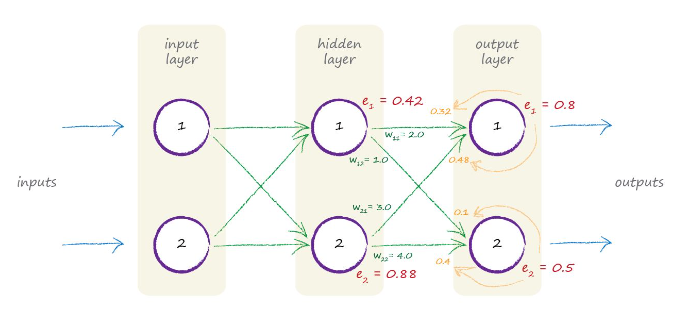
\includegraphics[width=0.7\linewidth]{images/TEMPbackpropagationErros1}
		\end{figure}
		
		
		\begin{figure}[H]
			\centering
			\caption{Retro-propagação da camada oculta para a entrada}
			\label{fig:backpropagationerros2}
			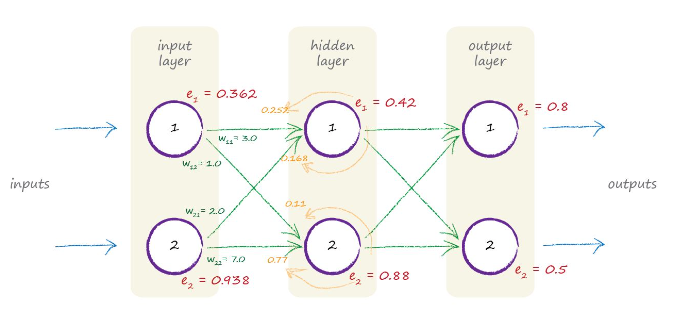
\includegraphics[width=0.7\linewidth]{images/TEMPbackpropagationErros2}
		\end{figure}
	
	\section{Retro-propagação II}
		\par Sendo uma rede neural um aproximador universal de funções, o algoritmo de retro-propagação será feito de forma que a taxa de variação dessa função (derivada) seja levado em conta. Especificamente, a função em questão, é o que se convencionou chamar função de custo ou de erro, que é um método para calcular o erro total que a rede produziu dada uma certa entrada, sendo assim, a função de custo também engloba a função de ativação ja que esta contribui para o erro, esse fato será importante mais a frente quando a derivada da mesma será necessária graças à regra da cadeia.
		
		\par Para melhor entender como a derivada da função de erro para uma rede neural deve ser tomada, é necessário primeiro entender o que é o vetor gradiente: O vetor gradiente é aquele que aponta para o maior crescimento da função dadas as derivadas parciais dos respectivos parâmetros da mesma. No caso de uma rede neural os parâmetros são os pesos que interliga cada neurônio que a compõem.
		
		\par Portanto se $f$ é uma função \ref{eq:function}  que contém os parâmetros $x_1, x_2, x_3$, por exemplo. Então o vetor gradiente da mesma será compostos pelas derivadas parciais de cada parâmetro \ref{eq:gradientVector}.

		\begin{equation}\label{eq:function}
			f(x_1, x_2, x_3)
		\end{equation}

		\begin{equation}\label{eq:gradientVector}
			\nabla f(x_1, x_2, x_3) = \begin{bmatrix}
				\dfrac{\delta f}{\delta x_1}  \\\\
				\dfrac{\delta f}{\delta x_2}  \\\\
				\dfrac{\delta f}{\delta x_3} 
			\end{bmatrix}
		\end{equation}
	
		\par Como já foi dito, o gradiente da função aponta para a direção dentro do domínio da função onde a mesma cresce mais rápido, no entanto, a intenção não é maximizar a função e sim minimiza-las, portanto, para que seja possível encontrar um mínimo da função, considera-se o valor oposto (negativo) do gradiente. Sendo assim, considerando que $X_t$ denota o valor atual  do parâmetro $X$ (que é um vetor) e  $X_{t+1}$ corresponde ao próximo valor que será fornecido a função $f$. O cálculo de $X_{t+1}$ se dará como mostrado na equação \ref{eq:nextX} .
	
			\begin{equation}\label{eq:nextX}
				X_{t+1} = X_t  - \eta . \nabla f(X_t)
			\end{equation}
	
			\par Onde $\eta$ é um coeficiente escalar \textbf{bastante pequeno} conhecido como \textbf{coeficiente de aprendizado} cujo valor geralmente está abaixo de 1 como 0.1, 0,3, etc.
			
			\par Ou, de forma mais explícita, combinando as equações \ref{eq:gradientVector} e \ref{eq:nextX} se tem a expressão \ref{eq:nextXII}.
			
			\begin{equation}\label{eq:nextXII}
				X_{t+1} = \begin{bmatrix}
					\dfrac{\delta f}{\delta {x[0]_t}}  \\\\
					\dfrac{\delta f}{\delta {x[1]_t}}  \\
					\vdots  \\
					\dfrac{\delta f}{\delta {x[n]_t}} 
				\end{bmatrix}  - \eta . \begin{bmatrix}
				\dfrac{\delta f}{\delta {x[0]_t}}  \\\\
				\dfrac{\delta f}{\delta {x[1]_t}}  \\
				\vdots  \\
				\dfrac{\delta f}{\delta {x[n]_t}} 
			\end{bmatrix}  
			\end{equation}
		
		\par O conteúdo acima apresentado ajudará no algoritmo de retro-propagação que, como já foi dito, considerará os pesos das sinapses da rede neural. É importante frisar que as entradas da rede neural e as respectivas saídas esperadas também serão importantes, já que, o valor da função de custo só pode ser calculado na existência desses dois valores.
		
		\par Considere a representação de uma rede neural.
		%TODO Fazer uma figura de uma rede neural totalmente conectada 3,2,3,2,2
			
		\begin{figure}[H]
			\centering
			\caption{Rede neural de três camadas escondidas, os pesos representados pelas variáveis $w_1, w_2, w_3$ na figura \ref{fig:3LayersNeuralNetwork} são alguns dos parâmetros da rede que devem ser ajustados para que hajam resultados satisfatórios.}
			\label{fig:3LayersNeuralNetwork}
			
\includegraphics[width=0.7\linewidth]{images/placeholder}
		\end{figure}
	
		\par Considere  para fins de exemplo o vetor de entrada \ref{eq:inputVector}, o vetor de saída \ref{eq:outputVector} e o vetor da saída desejada \ref{eq:targetVector}.
		
		\begin{equation}\label{eq:inputVector}
 		 X = \begin{bmatrix}
			 	1 \\
			 	0 \\
			 	2  
			 \end{bmatrix}
		\end{equation}
	
		\begin{equation}\label{eq:outputVector}
			O = \begin{bmatrix}
				-1 \\
				3 
			\end{bmatrix}
		\end{equation}
	
		\begin{equation}\label{eq:targetVector}
		T = \begin{bmatrix}
			1 \\
			0 
		\end{bmatrix}
		\end{equation}
		
		\par O vetor de entrada $X$ será processado pela rede produzindo um vetor de saída $O$, A função de custo usará os valores de $O$ e $T$ para calcular o custo total da rede para, dessa forma, ajustar seus parâmetros. A função de custo de uma rede pode ser das mais variadas, no entanto, para fins de entendimento usaremos o erro quadrática médio que, além de ser uma boa função de custo, se mostrará conveniente quando houver a necessidade de derivá-la.
		
		\par Para começar calcula-se o erro que é a diferença entre a saída desejada e a saída obtida pela rede como mostrado na equação \ref{eq:error}.
		
		\begin{equation}\label{eq:error}
			E0 = O - T
		\end{equation}
	
		\par Resultando nos valores:
		
		\begin{equation}\label{eq:outputVector}
			E0 = \begin{bmatrix}
					-1 \\
					3 
			\end{bmatrix}-\begin{bmatrix}
				1 \\
				0 
			\end{bmatrix} =\begin{bmatrix}
				-2 \\
				3 
			\end{bmatrix}
		\end{equation}
	
	\par Calculado o erro $E0$, passa-se ao cálculo do custo $E$ aplicando-se a soma dos quadrados de cada item do vetor de erros, dividindo o resultado por dois, como já foi dito essa divisão é apenas uma conveniência pois facilitará os cálculos no momento da derivação, $n$ é a quantidade de elementos no vetor de saída.
	
	\begin{equation}\label{eq:averageQuadError}
		E = \dfrac{1}{2.n}. \sum_{i=0}^{n}  (E_i)^2 = \dfrac{1}{2n} . (-2^2 + 3^2)  = \dfrac{1}{2.2} . (4 + 9) = \dfrac{1}{4} . 13 = \dfrac{13}{4} 
	\end{equation}


	\par Agora que o processo de cálculo de custo da rede foi explicado é necessário ter uma visão geral de como a rede será treinada:
	
	\begin{itemize}
		\item Preparar as entradas e as respectivas saídas esperadas para rede neural
		\item A partir do custo calculado calcular o gradiente dessa função de custo
		\item Ajustar os pesos e os \textit{bias} da rede em direção oposta ao gradiente calculado
		\item Repetir o processo até que uma condição de parada seja encontrada, muita das vezes essa será o custo máximo.
	\end{itemize}
	
	\par Tendo em mente essa visão geral, considere agora duas camadas $l - 1$ e $l$ de uma rede qualquer como mostrado na figura \ref{fig:layers}.
	
	\begin{figure}[H]
		\centering
		\caption{Duas camadas quaisquer de uma rede neural totalmente ligada, o neurônio $j$ pertence a camada $l -1$ e um neurônio $i$ pertence a camada $l$, dessa forma, o peso (ou peso sináptico) pertencente a camada $l$ que liga o neurônio $j$ ao neurônio $i$ é escrito como $w^l_{ij}$ }
		\label{fig:layers}
		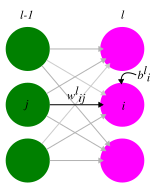
\includegraphics[width=0.5\linewidth]{images/layers}
	\end{figure}

	\par Representados como mostrado na figura \ref{fig:layers} e considerando $W^l$ como a representação de todos os pesos sinápticos pertencentes a camada $l$ essa notação proporciona uma representação matricial descrita na equação \ref{eq:weightsMatrix} onde $i$ é a linha e $j$ a coluna da matriz. De outra forma: Cada linha $i$ representa o correspondente neurônio da camada $l$ e cada coluna representa o correspondente neurônio da camada $l-1$ e, as intersecções, representam os pesos sinápticos que ligam um neurônimo ao outro. Os \textit{bias} $B^l$ da camada $l$ são representados em \ref{eq:biasVector}. 
	
	\begin{equation}\label{eq:weightsMatrix}
		W^l = \begin{bmatrix}
			\vdots && \vdots && \vdots && \vdots \\
			\hdots && w^l_{ij} && \hdots && \hdots \\
			\vdots && \vdots && \vdots && \vdots \\
			\vdots && \vdots && \vdots && \vdots \\
		\end{bmatrix}
	\end{equation}

	\begin{equation}\label{eq:biasVector}
		B^l = \begin{bmatrix}
			\vdots \\
			b^l_i  \\
			\vdots \\
			\vdots \\
		\end{bmatrix}
	\end{equation}

	\par Para que a rede neural tenha seus pesos sináptica os atualizados é necessário que a operação de \textit{feedforward} seja realizada afim de poderem ser calculados os erros da rede e consequentemente o seu custo.
	
	\begin{figure}[H]
		\centering
		\caption{Representação do \textit{feedforward}: $S^l_i$ é a soma das saídas vindas da camada $l-1$ ponderadas pelos respectivos pesos $ w^l_{ij}$ mais os \textit{bias} $B^l$ da camada $l$, $Z^l_i$ é um valor escalar resultante da aplicação de uma função de ativação sobre $S^l_i$}
		\label{fig:layersFeedforward}
		
\includegraphics[width=0.5\linewidth]{images/placeholder}
	\end{figure}

	\par A função de ativação, também conhecida como função de transferência, citada na figura \ref{fig:layersFeedforward} é representada na equação \ref{eq:activationFunction}.
	
	\begin{equation}\label{eq:activationFunction}
		Z^l_i = \sigma(S^l_i)
	\end{equation}
	
	\chapter{Paralelismo}
		\par 
		
		\chapter{Medidas dos tempos de execução do software}
		% TODO Fazer testes de execução e medir os tempos de classificassão e treinamento do softwares
		% perto sakr hotel em frente a BR, depois do balão
		
		
\end{apendicesenv}









